\documentclass[12pt,a4paper]{article}

\usepackage[a4paper,top=2.5cm,bottom=2.5cm,left=3cm,right=2.2cm]{geometry}
\usepackage{fontspec}
\usepackage{setspace}
\usepackage{titlesec}
\usepackage{enumitem}
\usepackage{hyperref}
\usepackage{xurl}
\usepackage{graphicx}
\usepackage{booktabs}
\usepackage{array}
\usepackage{caption}
\usepackage{amsmath}

\setmainfont{Times New Roman}
\setstretch{1.18}
\hypersetup{colorlinks=false,pdfborder={0 0 0}}

\titleformat{\section}
  {\normalfont\Large\bfseries}
  {\thesection}{0.8em}{}
\titleformat{\subsection}
  {\normalfont\large\bfseries}
  {\thesubsection}{0.8em}{}

\titlespacing*{\section}{0pt}{1.2em}{0.7em}
\titlespacing*{\subsection}{0pt}{1.0em}{0.45em}

\setlength{\parindent}{1.2cm}
\setlength{\parskip}{0.25em}
\emergencystretch=2em
\sloppy
\setlist[itemize]{leftmargin=1.8cm,itemsep=0.18em,topsep=0.25em}
\setlist[enumerate]{leftmargin=1.8cm,itemsep=0.18em,topsep=0.25em}
\newcommand{\codepath}[1]{\path{#1}}
\renewcommand{\arraystretch}{1.18}
\renewcommand{\refname}{References}

\begin{document}

\begin{titlepage}
  \thispagestyle{empty}
  \begin{center}
    \vspace*{0.6cm}
    {\Large\bfseries HANOI UNIVERSITY OF SCIENCE AND\\ TECHNOLOGY}

    \vspace{0.6cm}
    {\large\bfseries SCHOOL OF INFORMATION AND COMMUNICATIONS TECHNOLOGY}

    \vspace{0.9cm}
    \includegraphics[page=1,trim=83 510 100 150,clip,width=0.78\textwidth]{report_sample.pdf}

    \vspace{1.0cm}
    {\Large\bfseries INTERNSHIP REPORT}

    \vspace{0.7cm}
    {\LARGE\bfseries EBR-RAG: Multi-Agent Debate for\\ Retrieval-Augmented Generation on\\ Extreme Long-Context Videos}

    \vspace{1.0cm}
    {\large \textbf{Instructor:} Assoc. Prof. Dr. Lê Thanh Hương}

    \vspace{0.7cm}
    {\large \textbf{Student:} Nguyễn Tiến Thắng 20225530}

    \vfill
  \end{center}
\end{titlepage}

\begin{titlepage}
  \thispagestyle{empty}
  \begin{center}
    {\Large\bfseries Abstract}
  \end{center}

  \vspace{0.8cm}

  This internship report presents the implementation process of the project \textit{EBR-RAG: Multi-Agent Debate for Retrieval-Augmented Generation on Extreme Long-Context Videos} at NLP Lab. The main tasks include studying the overall architecture of a Video RAG system, analyzing the limitations of traditional question answering systems on long video data, investigating Graph-based RAG, improving graph construction with TM-Graph, developing a Multi-Agent Debate mechanism for the generation stage, and implementing an integrated pipeline from Ingestion to Generation. Within the experimental scope, the system was run on a LongerVideos subset consisting of three representative collections and was evaluated using the original baseline benchmark metrics together with RAGAS for the retrieval stage.

  The obtained results include a solid understanding of both foundational and advanced knowledge in Retrieval-Augmented Generation for multimodal data, successful integration of TM-Graph into the extraction process, development of a Multi-Agent Debate module to improve answer generation quality for long videos, and completion of experimental scripts for video ingestion, graph processing, generation evaluation using the baseline benchmark, and retrieval evaluation using RAGAS.

  \vspace{0.5cm}
  \noindent\textbf{Keywords:} Video RAG, EBR-RAG, TM-Graph, Multi-Agent Debate, Retrieval-Augmented Generation, long-context video question answering, RAGAS.
\end{titlepage}

\section{Introduction}

\subsection{Motivation}

Retrieval-Augmented Generation (RAG) is an important approach in modern question answering systems. Instead of requiring a large language model to memorize all knowledge in its parameters, RAG separates answer generation into two main stages: retrieving relevant information from an external knowledge source and generating an answer grounded in the retrieved information. This approach allows a system to update knowledge more flexibly, reduces dependence on the parametric memory of the model, and makes it easier to produce answers with explicit grounding.

In conventional text-based tasks, the knowledge base is usually divided into short text passages and then encoded into vectors for retrieval. However, when the task is extended to long video data, the problem becomes much more complex. A long video contains not only speech or subtitles, but also visual information, audio signals, actions, context, objects, characters, temporal development, and relations among events. These pieces of information may appear sparsely at different timestamps in the video, or across multiple videos within the same collection. Therefore, answering a question cannot rely only on a short text passage; it often requires evidence synthesis from multiple sources and multiple points in time.

Traditional question answering systems face several limitations when handling long video data. If the whole transcript or caption is fed into a language model, the computational cost becomes very high and the input may exceed the context window. If the system only uses dense retrieval over text chunks, it may miss indirect semantic relations or evidence that exists mainly in the visual channel. If the system retrieves only a few video segments close to the query, the answer may lack global context. In addition, one-shot generation can produce answers that are insufficiently verified, especially when the initial evidence is incomplete or noisy.

In this context, the topic \textit{EBR-RAG: Multi-Agent Debate for Retrieval-Augmented Generation on Extreme Long-Context Videos} was selected to study and extend VideoRAG for question answering over extreme long-context videos. The main approach combines three components: Video RAG for multimodal data processing, Graph-based RAG for modeling knowledge and relations among entities, and Multi-Agent Debate for improving answer generation through critique, evidence supplementation, and final synthesis.

\subsection{Internship Objectives and Scope}

The objective of the internship was to study, implement, and evaluate a pipeline extended from the VideoRAG baseline. The pipeline does not stop at retrieving relevant text passages or video segments; it also organizes evidence into a multi-step verification process before producing the final answer. During the internship, the focus was on understanding the existing system architecture, identifying possible improvement points, implementing new modules, and building experimental scripts for evaluation.

The scope of work included:
\begin{itemize}
  \item Studying the overall VideoRAG baseline architecture, including video ingestion, segmentation, transcript/caption generation, vector database construction, and knowledge graph construction.
  \item Analyzing the limitations of traditional QA/RAG systems on long video data, especially context loss, missing evidence, and hallucination in generation.
  \item Studying Graph-based RAG and the representation of video knowledge through entities, relations, and related segments.
  \item Improving graph construction with TM-Graph, focusing on reducing duplicate entities that are not merged across segments and mitigating missing entity extraction when required context appears in previous segments.
  \item Developing the EBR-RAG pipeline with evidence retrieval from three sources: text, graph, and visual segments.
  \item Developing a Multi-Agent Debate module for generation, including Generator, Critique Agent, Defender Agent, and Judge; the asymmetric information design keeps Critique more independent while allowing Defender to retrieve additional evidence to reduce hallucination.
  \item Completing experimental scripts for ingestion, ablation, generation evaluation using the original benchmark, and retrieval evaluation using RAGAS.
\end{itemize}

Because the internship had limited time and computational resources, this report focuses on research, design, integration, and evaluation on a representative LongerVideos subset. Generation is evaluated using the original baseline benchmark metrics, while retrieval is evaluated using RAGAS over the implemented ablation scenarios.

\section{Project Overview}

\subsection{Base System: VideoRAG}

The project is developed from the VideoRAG baseline, a Retrieval-Augmented Generation system designed for extreme long-context videos \cite{ren2025videorag}. The main idea of VideoRAG is to transform raw long videos into retrievable structures before answering queries. Instead of directly feeding the entire video into a model, the system first performs ingestion, extracts multimodal information, builds vector databases, and constructs a knowledge graph.

According to the baseline architecture, VideoRAG uses a dual-channel mechanism. On one side, the system builds a knowledge graph from text chunks to model relations among entities in the video. On the other side, it stores multimodal representations of video segments to support retrieval based on visual and textual context. Given a question, the system combines entity-based retrieval, text-based retrieval, and video feature retrieval to build an evidence set for generation.

In the current codebase, the central class is \codepath{videorag/videorag.py}. The \codepath{VideoRAG} class manages video ingestion, segment information storage, text chunk construction, vector database updates, entity extraction, and knowledge graph writing. The EBR-RAG project extends this class by adding the query mode \codepath{mode="EBR_RAG"}, which calls the new pipeline in \codepath{videorag/pipeline/EBR_RAG.py}.

\begin{figure}[h]
  \centering
  \includegraphics[width=0.92\textwidth]{VideoRAG.png}
  \caption{Overall VideoRAG architecture used as the baseline for the project.}
\end{figure}

\subsection{Dataset and Benchmark}

The main dataset referenced in the project is the LongerVideos benchmark from VideoRAG. This benchmark is designed to evaluate the ability to understand multiple long videos and answer open-ended questions. The dataset includes videos from several domains such as lecture, documentary, and entertainment. This makes it suitable for the goal of the project: evaluating RAG in a long-video environment with diverse topics and dispersed contexts.

Within the internship, experiments were conducted on three collections, selected to represent three categories and to provide a reasonable number of questions:
\begin{itemize}
  \item \codepath{6-daubechies-wavelet-lecture}: lecture domain, 4 videos, 25 questions.
  \item \codepath{11-primetime-emmy-awards}: entertainment domain, 3 videos, 17 questions.
  \item \codepath{19-jeff-bezos}: documentary domain, 3 videos, 34 questions.
\end{itemize}

In total, the evaluation subset contains 10 videos and 76 questions. Using these three collections makes it possible to run ingestion, retrieval, debate, and evaluation repeatedly while still covering different data domains.

\subsection{Models and Tools}

The project uses \codepath{gpt-4o-mini} as the main LLM for generation, entity extraction, entity resolution, debate, and evaluation-related prompts. Text embeddings use \codepath{text-embedding-3-small} with dimension 1536. Visual captioning uses MiniCPM-V 2.6 int4, while ASR uses faster-distil-whisper-large-v3. Visual retrieval over video segments uses ImageBind embeddings.

For storage, the system uses JSON key-value storage, vector databases for text chunks/entities/video segments, and a graph storage layer for the knowledge graph. The main code modules include:

\begin{center}
\begin{tabular}{p{0.32\textwidth}p{0.56\textwidth}}
\toprule
\textbf{Component} & \textbf{Role in the project} \\
\midrule
\codepath{videorag/videorag.py} & Main class for ingestion, storage initialization, and query dispatch. \\
\codepath{videorag/_op.py} & Core functions for chunking, entity extraction, graph construction, and retrieval. \\
\codepath{videorag/pipeline/EBR_RAG.py} & EBR-RAG orchestrator, including initial retrieval, evidence budgeting, query-aware refinement, and debate invocation. \\
\codepath{videorag/debate/} & State, evidence types, and debate manager for Multi-Agent Debate. \\
\codepath{videorag/tools/} & Retrieval tools for text, graph, and visual evidence. \\
\codepath{reproduce/run_ablation_matrix.py} & Script for running EBR-RAG ablation scenarios and saving answers in a baseline-compatible format. \\
\codepath{reproduce/quantitative_comparison/} & Directory containing quantitative evaluation scripts, including EBR-RAG evaluation and RAGAS retrieval evaluation. \\
\bottomrule
\end{tabular}
\captionof{table}{Main source code structure used in the project.}
\end{center}

\subsection{Main References}

During the project, several papers directly related to Video RAG, Graph-based RAG, and Multi-Agent Debate were studied. This report cites only the most important references to keep the background concise.

\begin{center}
\small
\begin{tabular}{p{0.28\textwidth}p{0.54\textwidth}}
\toprule
\textbf{Reference} & \textbf{Role in the project} \\
\midrule
\textit{VideoRAG: Retrieval-Augmented Generation with Extreme Long-Context Videos} \cite{ren2025videorag} & Baseline paper and main benchmark for the project. \\
\textit{Improving Factuality and Reasoning in Language Models through Multiagent Debate} \cite{du2023multiagent} & Basis for designing Generator, Critique, Defender, and Judge roles in generation. \\
\textit{Breaking the Martingale Curse: Multi-Agent Debate via Asymmetric Cognitive Potential Energy} \cite{liu2026martingale} & Theoretical basis for asymmetric information among agents, especially not allowing Critique Agent to directly see the full evidence pool by default. \\
\textit{Removal of Hallucination on Hallucination: Debate-Augmented RAG} \cite{hu2025drag} & Closely related work in text RAG, using debate and asymmetric information roles to reduce hallucination caused by retrieval noise. \\
\textit{Vgent: Graph-based Retrieval-Reasoning-Augmented Generation For Long Video Understanding} \cite{shen2025vgent} & Related work on graph-based long-video RAG, different from this project because it focuses on graph retrieval-reasoning for LVLMs rather than improving entity extraction and graph construction inside VideoRAG. \\
\bottomrule
\end{tabular}
\captionof{table}{Main references used in the report.}
\end{center}

\subsection{Hardware}

The VideoRAG baseline is designed to process hundreds of hours of video on a 24GB GPU, such as an NVIDIA RTX 3090. In this internship project, video ingestion and captioning remain the most resource-consuming steps because they require video splitting, audio processing, VLM captioning, and video feature encoding. Therefore, experiments in the internship were limited to three representative LongerVideos collections so that ingestion, ablation, RAGAS retrieval evaluation, and generation benchmark evaluation could be completed within the available resources.

\section{Methodology}

\subsection{Long-Context Video RAG Problem}

The Long-Context Video RAG problem can be described as follows: given a set of long videos and a natural language question, the system must retrieve relevant evidence from the video content and generate a grounded answer. Unlike text-only RAG, evidence in video may appear as transcript, caption, visual segment, graph entity, or relations among entities. Therefore, the pipeline must process data through multiple stages before it can answer a question.

In this project, the pipeline is divided into three main stages:
\begin{enumerate}
  \item \textbf{Ingestion}: transform raw video into short segments, generate transcripts using ASR, generate captions using a vision-language model, store segment information, split text chunks, encode chunks/entities/video segments into vector databases, and construct the knowledge graph.
  \item \textbf{Retrieval}: when a question is received, retrieve evidence from text chunks, graph, and visual segments.
  \item \textbf{Generation}: generate an answer based on evidence. In EBR-RAG, this stage is extended into Multi-Agent Debate to improve verification.
\end{enumerate}

This separation allows the system to process long videos in a structured manner. Instead of feeding the whole video into a model, the system transforms videos into retrievable indexes. When a question arrives, only the most relevant segments are passed to generation, reducing cost and improving grounding.

\subsection{Ingestion Process}

In the VideoRAG baseline, ingestion is not only the step of reading raw videos. It is the full process of transforming long videos into retrievable structures. Each video is first split into short segments with a default length of 30 seconds. Each segment keeps its timestamp, video name, and segment index, allowing later evidence to be traced back to its original position in the video.

After segmentation, the system creates two main content descriptions. For the audio channel, ASR with faster-distil-whisper-large-v3 is used to generate transcripts. For the visual channel, MiniCPM-V 2.6 int4 receives sampled frames from the segment, together with the transcript, and generates a caption describing the visual content. Transcript and caption are merged into segment text, which becomes the central textual representation of the segment.

From segment text, ingestion builds the indexes used for retrieval. Segment contents are split into text chunks and encoded with text embeddings into the chunks VDB. In parallel, the system extracts entities and relations from chunks to construct a knowledge graph. In this graph, nodes represent entities or concepts, edges represent relations among entities, and \codepath{source_id} links nodes/edges back to source chunks and segments. Entities are also encoded and stored in the entity VDB to support entity retrieval when a query is received.

In addition to text and graph channels, ingestion also builds a visual index. Video segments are encoded by ImageBind and stored in the video segment feature VDB. Therefore, when a question contains visual signals or requires locating a specific action/scene, the system can directly retrieve relevant segments using cross-modal embeddings. After ingestion, the baseline pipeline has three main retrieval sources: text chunks, knowledge graph/entity VDB, and visual segment VDB.

\subsection{Limitations of Traditional QA/RAG on Long Videos}

After studying the baseline pipeline, two main limitations were identified. The first limitation lies in graph construction. Entity extraction in the baseline is performed per chunk, and many chunks are processed independently for speed. This can cause \textit{entity fragmentation}: the same real-world object, such as a person, organization, or concept, appears in multiple segments but is stored as multiple graph nodes due to small differences in naming or description. As a result, knowledge about the same entity is scattered, making graph retrieval less effective at expanding to related segments.

Still within graph construction, parallel chunk-level extraction reduces the ability to use before-after context. A single chunk may contain pronouns, abbreviated names, or an event introduced in a previous segment. Without temporal context, the model may miss entities, produce poor entity descriptions, or miss important relations. This gap motivated TM-Graph: bringing short-term memory of recently seen entities into extraction and entity resolution to reduce graph fragmentation and improve entity/relation completeness.

The second limitation lies in generation. After retrieval, the baseline often lets the model directly generate an answer from the initial evidence. For long videos, evidence may be incomplete, noisy, or only partially cover the question. Therefore, a one-shot answer may be insufficiently rigorous, may fail to check assumptions, and may be overly confident. This gap motivated EBR-RAG with Multi-Agent Debate: generating a draft, critiquing it, retrieving additional evidence when needed, and letting Judge synthesize the final answer.

\subsection{EBR-RAG Pipeline}

The EBR-RAG pipeline is implemented in \codepath{videorag/pipeline/EBR_RAG.py}. It is the orchestrator called from \codepath{VideoRAG.aquery()} when \codepath{param.mode == "EBR_RAG"}. The goal of the pipeline is to construct a multi-source evidence pool, refine evidence when needed, and pass it to Multi-Agent Debate for final answer generation.

\begin{figure}[h]
  \centering
  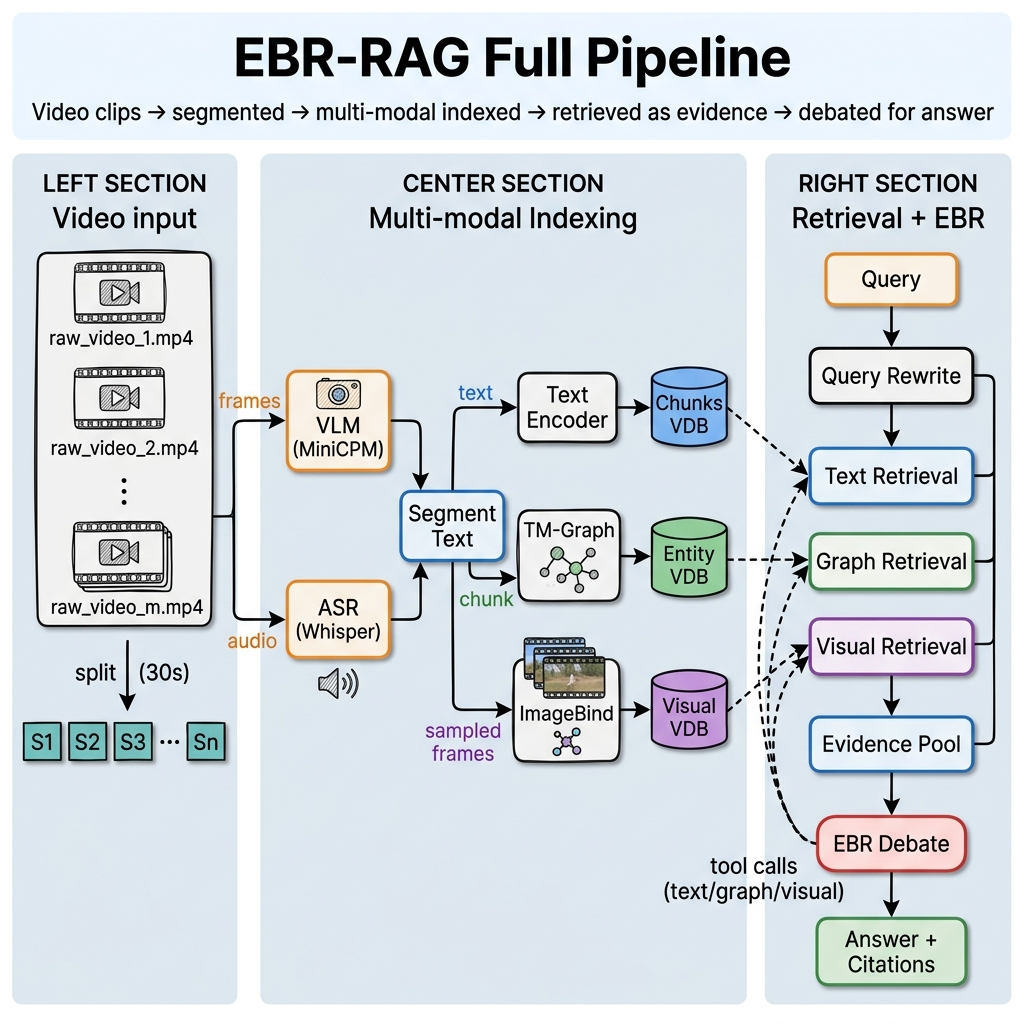
\includegraphics[width=0.95\textwidth]{report_assets/diagrams/01_full_pipeline.png}
  \caption{Overall EBR-RAG pipeline from ingestion and retrieval to generation.}
\end{figure}

At the beginning, the pipeline builds handles to existing storage components in the \codepath{VideoRAG} object: chunks VDB, text chunks, entities VDB, knowledge graph, video segment feature VDB, video segments, video path database, and caption model. It then runs three retrieval branches:
\begin{itemize}
  \item \textbf{Text retrieval}: calls \codepath{search_text_evidence()} to rewrite the query, retrieve dense chunks, and expand evidence through entity/graph information.
  \item \textbf{Graph retrieval}: calls \codepath{search_graph_evidence()} to find related entities, obtain node data from the graph, and find related segments.
  \item \textbf{Visual retrieval}: calls \codepath{search_visual_segment()} to rewrite the query toward visual intent and retrieve video segments from the multimodal VDB.
\end{itemize}

In the current configuration, each branch uses \codepath{top_k=8}. Evidence from the three branches is merged, deduplicated by \codepath{_dedup_evidence()}, and limited to an initial budget of 24 items. This pre-refinement budget is necessary because query-aware re-captioning with a VLM is expensive. After refinement, the pipeline sets a universal cap of \codepath{24 + max_rounds * 3}. With \codepath{max_rounds=3}, the maximum evidence pool is 33 items: 24 initial evidence items and up to 9 additional evidence items during debate.

More specifically, EBR-RAG treats retrieval as evidence pool construction rather than retrieving a single context for the LLM. Text retrieval returns \codepath{text EvidenceItem} objects from the dense chunk VDB, with \codepath{entity_boost=True} allowing entity/graph expansion when needed. Graph retrieval returns \codepath{entity EvidenceItem} objects, including node information, entity description, and related segments/chunks from the graph. Visual retrieval returns \codepath{segment EvidenceItem} objects from the ImageBind-encoded video segment feature VDB. These three sources complement each other: text retrieval is strong for keyword-rich questions, graph retrieval is strong for entity/relation questions, and visual retrieval is useful when the question depends on scenes, actions, or visual signals.

For \codepath{segment} evidence, EBR-RAG adds a query-aware refinement step. The pipeline first extracts keywords from the question, then calls \codepath{retrieved_segment_caption()} to re-caption selected segments with MiniCPM-V. The number of sampled frames in refinement is controlled by \codepath{fine_num_frames_per_segment}, which defaults to 15 in the configuration. The new caption replaces the old snippet and the metadata is marked as \codepath{refined=True}. The goal is to make visual evidence more query-focused instead of using only the generic caption produced during ingestion.

\begin{center}
\begin{tabular}{p{0.22\textwidth}p{0.28\textwidth}p{0.38\textwidth}}
\toprule
\textbf{Stage} & \textbf{Module} & \textbf{Function} \\
\midrule
Initial retrieval & \codepath{text_tools.py} & Dense text retrieval with entity/graph expansion. \\
Initial retrieval & \codepath{graph_tools.py} & Retrieve graph entities and related segments. \\
Initial retrieval & \codepath{vision_tools.py} & Retrieve video segments with visual/cross-modal embeddings. \\
Evidence processing & \codepath{EBR_RAG.py} & Deduplication, evidence budget, and query-aware segment refinement. \\
Generation & \codepath{debate_manager.py} & Generator, Critique, Defender, and Judge produce the final answer. \\
\bottomrule
\end{tabular}
\captionof{table}{Main components in the EBR-RAG pipeline.}
\end{center}

\subsection{EvidenceItem Design}

To allow different retrieval sources to be used together in debate, the project defines the \codepath{EvidenceItem} type. Each evidence item contains fields such as \codepath{id}, \codepath{type}, \codepath{score}, \codepath{snippet}, \codepath{source}, \codepath{video_name}, \codepath{segment_index}, \codepath{time_range}, and \codepath{metadata}. The three main evidence types are \codepath{text}, \codepath{entity}, and \codepath{segment}.

This normalization allows debate agents to ignore whether evidence comes from dense retrieval, graph retrieval, or visual retrieval. An agent only needs to read the snippet, source, score, and provenance information. For video segment evidence, fields such as video name, segment index, and time range allow the final answer to refer back to the position in the video. This is a prerequisite for citation and evidence verification.

When inserted into prompts, evidence is formatted into blocks containing \codepath{id}, \codepath{type}, \codepath{score}, \codepath{source}, \codepath{video/time} if available, and \codepath{snippet}. Keeping the \codepath{id} in the prompt allows Judge to generate citations by evidence id, and the system can verify whether the cited id exists in the evidence pool. For multiple-choice questions, the pipeline detects options by regex; Generator and Judge then use MCQ-specific prompts, while open-ended questions use open-ended prompts.

\subsection{TM-Graph for Graph Construction}

One main task in the internship was designing and integrating TM-Graph into graph construction. Unlike baseline graph construction, TM-Graph does not treat each chunk as a fully independent unit. Instead, it processes chunks in temporal order and maintains a short-term memory of recently seen entities. This memory is injected into the extraction prompt as additional context, helping the model recognize previously mentioned entities and create more consistent nodes/relations.

TM-Graph aims to improve graph quality in long videos, especially for two common errors in independent chunk-level extraction. First, the same person, organization, or concept may appear multiple times across segments but be stored as different entities, fragmenting the graph. Second, when a chunk lacks enough context, the model may miss an entity or produce a poor description, even though supporting information appeared in previous segments. TM-Graph addresses these issues with short-term memory: recently resolved entities are inserted into the prompt as memory context, and new entities are compared against both memory and the global entity VDB before deciding whether to merge or create a new node.

\begin{figure}[h]
  \centering
  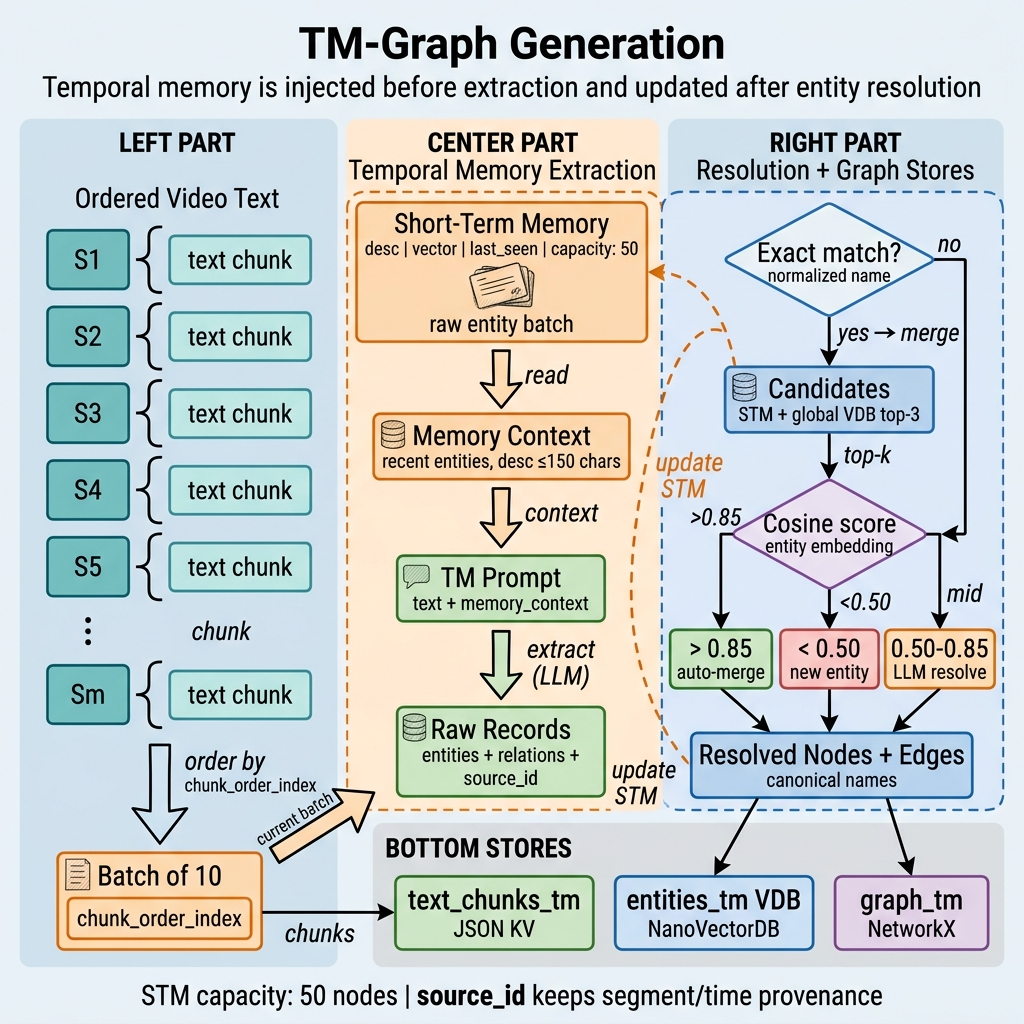
\includegraphics[width=0.95\textwidth]{report_assets/diagrams/03_tm_graph.png}
  \caption{TM-Graph construction with short-term memory for entity extraction and entity resolution.}
\end{figure}

The input of TM-Graph is the set of \codepath{text chunks} created during ingestion. Each chunk contains merged transcript/caption content, a list of \codepath{video_segment_id}, the number of tokens, and \codepath{chunk_order_index}. Unlike the baseline, chunks are first sorted in ascending order of \codepath{chunk_order_index}. This turns the chunk stream into an approximate temporal sequence of the video, allowing entity information from earlier segments to be carried to later segments.

TM-Graph processes chunks in batches with \codepath{batch_size=10}. Within a batch, chunks are still sent to the LLM in parallel to preserve processing speed; however, all chunks in the same batch receive the same \textit{memory context} created from the state before that batch. After the current batch is complete, entity/relation results are used to update memory for the next batch. In other words, TM-Graph uses a \textit{batch-sequential} strategy: parallel within a short range, but sequential over time at the batch level.

Short-term memory is stored as a mapping from \codepath{resolved_name} to \codepath{description}, \codepath{last_seen}, and an embedding vector if available. The \codepath{description} field is the representative description of the entity. The \codepath{last_seen} field records the latest batch in which the entity appeared and acts as a temporal recency signal. The vector embedding is computed from the string \codepath{name: description} and is used for semantic matching when deciding whether a new entity is the same as a previous one.

The memory context inserted into the prompt does not contain the whole graph. It contains only recently seen entities, formatted under \textit{Short-Term Memory (Recently seen entities)} as a list of \codepath{name: description} lines. Each description is truncated to at most 150 characters to reduce token usage and avoid overwhelming the extraction prompt. This design is intentional: in long videos, entities that appeared in nearby previous segments are usually more relevant than entities that appeared far away. Therefore, short-term memory works as a temporal context window rather than an unlimited global memory.

After the LLM extracts entities/relations from each chunk, TM-Graph does not immediately write raw nodes into the graph. Raw entities in the batch are first grouped by name, then entity resolution is performed. For each new entity, the system creates a query string \codepath{raw_name: description}. Entity names are normalized by lowercasing, stripping common articles or prefixes such as \codepath{the}, \codepath{a}, \codepath{an}, \codepath{mr.}, and \codepath{dr.}, and removing organization suffixes such as \codepath{inc.}, \codepath{llc}, and \codepath{corp}. If the normalized name matches an entity in short-term memory, the new entity is directly merged.

If there is no exact or normalized match, candidate entities are collected from two sources. The first source is the current short-term memory. The second source is the global entity VDB: the system queries the entity VDB with \codepath{raw_name: description} using \codepath{top_k=3}, then retrieves the corresponding graph node to obtain its description. Combining these sources allows TM-Graph to handle both recently appearing entities and older entities that were evicted from memory.

For the collected candidates, TM-Graph computes cosine similarity between the embedding of the new entity and the embedding of each candidate in memory. If the highest score is greater than \codepath{0.85}, the system automatically merges the new entity into that candidate. If the highest score is lower than \codepath{0.5}, the entity is treated as new. The range from \codepath{0.5} to \codepath{0.85} is uncertain; the system keeps up to the \codepath{top 5} candidates to save tokens and calls an LLM resolution prompt. The prompt asks the LLM to return the exact candidate name if the entities are the same character/object/concept, or \codepath{NONE} otherwise.

After mapping \codepath{raw_name} to \codepath{resolved_name}, TM-Graph updates three types of information. First, raw nodes are grouped under \codepath{resolved_nodes[resolved_name]} so that descriptions, types, and source ids can later be merged. Second, short-term memory updates \codepath{last_seen=current_time}; if the entity is new or has no vector, it is added to the embedding update list. Third, relations in the batch are remapped using resolved names; if source and target become the same after resolution, the edge is skipped to avoid meaningless self-loops.

Short-term memory is limited by \codepath{max_memory_nodes=50}. When the number of entities exceeds this threshold, the system sorts entities by \codepath{last_seen} and removes the oldest ones. Removing the oldest nodes from memory does not delete them from the graph or entity VDB; they are only removed from the short-term context for subsequent batches. This avoids overly long prompts, reduces noise, and helps the LLM focus on entities likely to be related to the current segment. If an old entity reappears after many segments, the global entity VDB can still retrieve it as a candidate for merging.

At the end, resolved nodes are written into the knowledge graph through node merging. If a node already exists, the system merges \codepath{entity_type}, concatenates and summarizes \codepath{description}, and merges \codepath{source_id} to preserve provenance to source chunks. For edges, the system merges relation descriptions, sums \codepath{weight}, and merges \codepath{source_id}. The entity VDB is then updated using \codepath{entity_name + description}. The final output of TM-Graph is a knowledge graph with reduced entity fragmentation, an updated entity VDB, and relations remapped to more consistent entity names.

Experimentally, TM-Graph is evaluated through ablation. \textit{Full Framework} uses both TM-Graph and Multi-Agent Debate, while \textit{Baseline with Debate} keeps debate but uses the baseline graph. Comparing these scenarios separates the effect of TM-Graph from the effect of Multi-Agent Debate. RAGAS retrieval evaluation also compares \codepath{tm_graph} and \codepath{baseline_graph} through context precision and context recall.

\subsection{Multi-Agent Debate for Generation}

Multi-Agent Debate is the most important extension of EBR-RAG in the generation stage. Instead of letting a model directly generate an answer from initial evidence, the pipeline organizes generation into multiple steps: draft, critique, refinement, and judgment. This design is inspired by multi-agent debate, where multiple models or roles critique each other over several rounds to improve factuality and reasoning \cite{du2023multiagent}. It is suitable for long-video QA because evidence may be incomplete at first, and the answer needs to be checked before finalization.

\begin{figure}[h]
  \centering
  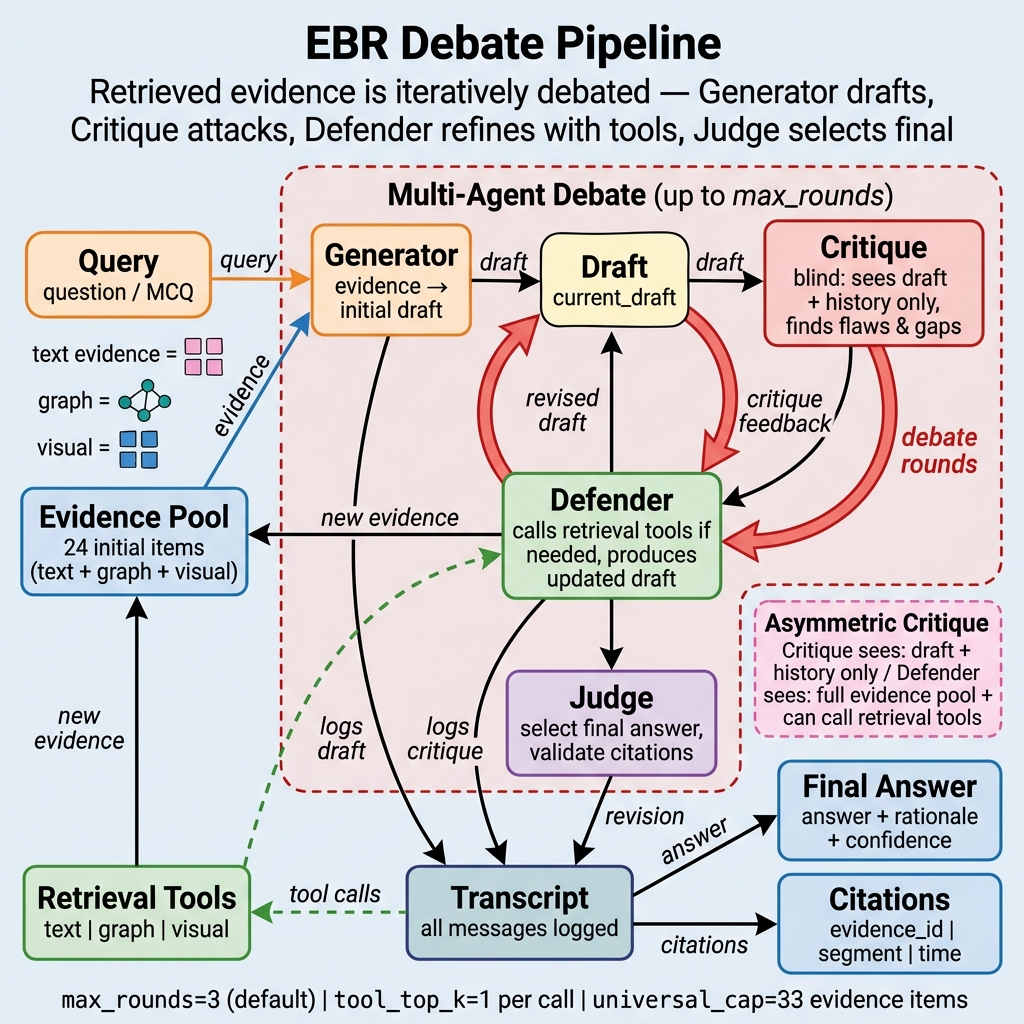
\includegraphics[width=0.95\textwidth]{report_assets/diagrams/02_ebr_debate.png}
  \caption{Multi-Agent Debate process in EBR-RAG.}
\end{figure}

In the current design, debate is organized as sequential refinement with clear roles:
\begin{enumerate}
  \item \textbf{Generator}: creates the initial draft based on the evidence pool.
  \item \textbf{Critique Agent}: analyzes the draft to find weaknesses, evidence gaps, or possible hallucination.
  \item \textbf{Defender Agent}: responds to critique, calls tools when needed to find additional evidence, and updates the draft.
  \item \textbf{Judge}: reads the refinement transcript and latest evidence pool to produce the final answer.
\end{enumerate}

Defender can call three retrieval tools: \codepath{search_text_evidence}, \codepath{search_graph_evidence}, and \codepath{search_visual_segment}. During debate, each tool call is limited to \codepath{top_k=1} to control cost and prevent the evidence pool from growing too large. Each round has a limited number of tool calls, while the state records \codepath{rounds_run} and \codepath{tool_calls_made} for observability and ablation.

At the parameter level, all roles use \codepath{gpt-4o-mini} but with different temperatures. Generator uses \codepath{0.5}, flexible enough to synthesize an initial answer from multiple evidence items. Critique uses \codepath{0.6}, slightly higher to find alternative critique angles and logical gaps. Defender uses \codepath{0.4}, lower than Critique because its task is to revise the draft and stay close to evidence. Judge uses \codepath{0.1} to make the final answer more stable. \codepath{QueryParam} sets \codepath{max_rounds=2} by default; in the full/debate experiments, it is usually set to 3.

In each round, Critique is called first. Its input includes the query, current draft, and recent refinement history, but by default it does not receive the evidence pool directly. This is the asymmetric information design of EBR-RAG: Critique checks the rigor of reasoning and detects hallucination from the answer itself, instead of reading the same evidence pool as Generator. If Critique identifies a gap, Defender is the agent allowed to read the evidence pool and call tools to add evidence. This separates the two behaviors: detecting problems and fixing them through retrieval.

Defender receives the query, current draft, critique feedback, and current evidence pool. In one round, Defender can make up to \codepath{max_calls=3} tool calls. The whole debate also tracks \codepath{tool_calls_made} with a safety limit of 25, and tool-calling stops when the evidence pool reaches the cap. Each tool call retrieves only \codepath{top_k=1}; therefore, with \codepath{max_rounds=3}, Defender can add up to about 9 new evidence items. New evidence is refined if it is a segment and appended to the shared evidence pool. After adding evidence or deciding no tool is needed, Defender produces an \textit{Updated Draft}; if this section exists and is sufficiently long, it replaces the old draft for the next round.

Judge is the final step. Judge reads not only the last draft, but also the compacted refinement transcript and latest evidence pool. The transcript keeps up to the latest 50 messages to avoid overly long prompts while retaining debate content. For open-ended questions, Judge returns the final answer and a default rationale; for multiple-choice questions, Judge is asked to return JSON, which is parsed with robust JSON extraction. Citations, if any, are cross-checked against valid evidence ids in the pool. Therefore, EBR-RAG returns not only an answer, but also metadata for analysis: answer, rationale, confidence, citations, transcript, evidence, number of rounds, and number of tool calls.

A key design choice is that Critique Agent does not receive the full evidence pool by default. It mainly sees the draft and refinement history to evaluate logical flaws, reasoning gaps, or hallucination signals. The reason is that if all agents see the same noisy evidence, debate may converge quickly to the same mistake. \textit{Breaking the Martingale Curse} analyzes correlated errors in multi-agent debate and argues that information asymmetry/cognitive potential can help avoid collective reinforcement of errors \cite{liu2026martingale}. In RAG, DRAG also uses asymmetric information roles and adversarial debate to reduce errors caused by retrieval noise \cite{hu2025drag}. Therefore, EBR-RAG keeps Critique as a relatively independent critic; the \textit{Critique with Evidence} ablation enables evidence access to test this design.

\subsection{Ablation Configuration}

To evaluate the contribution of each component, the project defines an ablation matrix in \codepath{reproduce/run_ablation_matrix.py}. The main scenarios are:

\begin{center}
\begin{tabular}{p{0.28\textwidth}p{0.58\textwidth}}
\toprule
\textbf{Scenario} & \textbf{Meaning} \\
\midrule
Full Framework & Uses both TM-Graph and full Multi-Agent Debate. \\
Baseline with Debate & Uses the baseline graph while keeping Multi-Agent Debate, to measure the separate effect of TM-Graph. \\
w/o Debate & Uses TM-Graph but sets \codepath{max_rounds=0}, to measure the effect of debate. \\
Critique with Evidence & Allows Critique to see evidence, to study the role of evidence access in critique. \\
Defender No Tools & Disables Defender tool-calling, to measure the effect of retrieving additional evidence during refinement. \\
\bottomrule
\end{tabular}
\captionof{table}{Ablation scenarios prepared in the project.}
\end{center}

The ablation script uses \codepath{return_detailed=True} to obtain dictionary output from EBR-RAG, checks that the answer is non-empty, and saves answers in a format compatible with \codepath{reproduce/all_answers}. This allows EBR-RAG results to be passed through the same evaluation pipeline as the baseline systems.

\subsection{Evaluation Configuration}

Evaluation is designed in two directions to separate retrieval quality from answer generation quality. The first direction evaluates generation using the original VideoRAG benchmark metrics. Scripts in \codepath{reproduce/quantitative_comparison/} convert answers from each method into the same baseline-compatible format and then use the benchmark evaluation process to compare against reference systems such as NaiveRAG or VideoRAG baseline. This answers the question: after the full retrieval and generation pipeline, is the final answer correct, complete, and competitive with the baseline?

The second direction evaluates retrieval separately using RAGAS. Retrieval is separated from generation because an incorrect answer may result from missing context, noisy evidence, or generation errors. RAGAS measures the evidence pool before Judge produces the final answer. The two main metrics in this project are \textit{context precision} and \textit{context recall}.

For a question, assume the system retrieves an ordered list of contexts $C = [c_1, c_2, ..., c_K]$. RAGAS marks each context $c_k$ as relevant or irrelevant to the question/ground truth, denoted by $v_k \in \{0, 1\}$. Context precision is computed as average precision:

\[
\mathrm{ContextPrecision@K} =
\frac{1}{\sum_{k=1}^{K} v_k}
\sum_{k=1}^{K}
\left(
\frac{\sum_{i=1}^{k} v_i}{k}
\right)
v_k
\]

In this formula, $\frac{\sum_{i=1}^{k} v_i}{k}$ is precision at position $k$. If relevant contexts are ranked early, context precision is high. This metric reflects the noise level and ranking quality of the evidence list.

Context recall measures how well retrieved contexts cover the information needed to answer the question. RAGAS usually decomposes the ground truth/reference into statements or information units and checks how many can be inferred from the retrieved contexts. The intuition can be written as:

\[
\mathrm{ContextRecall} =
\frac{
\left|\{s \in S_{\mathrm{ref}} \mid s \text{ is supported by } C\}\right|
}{
\left|S_{\mathrm{ref}}\right|
}
\]

Here, $S_{\mathrm{ref}}$ is the set of necessary statements in the reference answer. If the system retrieves many correct evidence items but misses the decisive segment, context recall remains low. This metric is especially important for long-context video QA, where answers may depend on a small segment far away in the video or on multiple dispersed segments.

The script \codepath{ragas_ablation_retrieval_eval.py} runs this evaluation. For each question in the LongerVideos subset, it runs each ablation scenario, collects the initial evidence, converts \codepath{EvidenceItem} objects into text contexts, combines them with the question and ground truth, and calls RAGAS. The generated outputs include \codepath{ragas_retrieval_rows.jsonl}, \codepath{ragas_retrieval_scores.jsonl}, \codepath{ragas_retrieval_scores.csv}, \codepath{ragas_retrieval_summary.json}, \codepath{ragas_retrieval_summary.csv}, and \codepath{ragas_retrieval_summary.md}. Results are aggregated by scenario to directly compare TM-Graph with the baseline graph and to compare debate variants in the retrieval stage.

\section{Results and Experiments}

\subsection{Experimental Setup}

The current experimental setup focuses on three representative LongerVideos collections: \codepath{6-daubechies-wavelet-lecture}, \codepath{11-primetime-emmy-awards}, and \codepath{19-jeff-bezos}. These collections represent lecture, entertainment, and documentary domains respectively, with a total of 10 videos and 76 questions. Each collection has its own working directory in \codepath{longervideos/videorag-workdir/}, which separates ingested data, graph, vector databases, and cache.

The LLM configuration for ingestion and evaluation uses \codepath{gpt-4o-mini}; text embedding uses \codepath{text-embedding-3-small} with dimension 1536. Visual captions are generated by MiniCPM-V 2.6 int4, ASR uses faster-distil-whisper-large-v3, and visual retrieval uses ImageBind embeddings for video segments. Retrieval parameters are unified at \codepath{top_k=8} for the initial EBR-RAG retrieval. For debate, the default ablation configuration uses \codepath{max_rounds=3}; the \textit{w/o Debate} scenario sets \codepath{max_rounds=0}. Defender can call tools to retrieve additional evidence except in the \textit{Defender No Tools} scenario.

\begin{center}
\begin{tabular}{p{0.36\textwidth}p{0.46\textwidth}}
\toprule
\textbf{Component} & \textbf{Current configuration} \\
\midrule
Embedding model & \codepath{text-embedding-3-small}, dimension 1536 \\
LLM generation/debate & \codepath{gpt-4o-mini} \\
Initial text top-k & 8 \\
Initial graph top-k & 8 \\
Initial visual top-k & 8 \\
Initial evidence budget & 24 items \\
Default debate rounds & 3 \\
Debate tool top-k & 1 item per call \\
Retrieval evaluation & RAGAS context precision/recall \\
Generation evaluation & Original benchmark metrics \\
\bottomrule
\end{tabular}
\captionof{table}{Main experimental configuration of EBR-RAG.}
\end{center}

\subsection{Retrieval Evaluation Results}

Retrieval evaluation answers the question: do TM-Graph and pipeline variants help retrieve more appropriate contexts? RAGAS is used because it can measure context quality independently of final answer quality. The two main metrics are context precision and context recall. The results below are computed on 76 questions from the three ingested LongerVideos collections, with an average of 8 contexts per question.

\begin{center}
\scriptsize
\setlength{\tabcolsep}{3pt}
\begin{tabular}{p{0.22\textwidth}p{0.15\textwidth}p{0.06\textwidth}p{0.10\textwidth}p{0.14\textwidth}p{0.13\textwidth}}
\toprule
\textbf{Method} & \textbf{Retrieval Config} & \textbf{N} & \textbf{Avg Contexts} & \textbf{Context Precision} & \textbf{Context Recall} \\
\midrule
Full Framework & TM-Graph & 76 & 8.00 & 0.5694 & 0.1140 \\
Baseline with Debate & Baseline Graph & 76 & 8.00 & 0.5640 & 0.0826 \\
w/o Debate & TM-Graph & 76 & 8.00 & 0.5916 & 0.0994 \\
Critique with Evidence & TM-Graph & 76 & 8.00 & 0.5812 & 0.1055 \\
Defender No Tools & TM-Graph & 76 & 8.00 & 0.5834 & 0.0682 \\
\bottomrule
\end{tabular}
\captionof{table}{RAGAS retrieval results on LongerVideos collections 6, 11, and 19.}
\end{center}

Full Framework achieves context recall 0.1140, higher than Baseline with Debate using the baseline graph at 0.0826. The absolute increase is 0.0314, equivalent to about 38.1\%. Meanwhile, context precision is 0.5694 for Full Framework and 0.5640 for Baseline with Debate. This indicates that TM-Graph mainly improves evidence coverage rather than drastically changing context ranking precision.

The \textit{w/o Debate} scenario achieves the highest precision, 0.5916, but recall is 0.0994, lower than Full Framework by 0.0146. This suggests that keeping only initial contexts may make the evidence list cleaner, but does not cover as much information as debate with Defender evidence supplementation. \textit{Defender No Tools} has the lowest recall, 0.0682, which is 0.0458 lower than Full Framework, showing the clear importance of Defender tool-calling. \textit{Critique with Evidence} has precision 0.5812 but recall 0.1055, lower than Full Framework; this matches the asymmetric information design where Critique remains independent and Defender handles evidence-grounded correction.

\subsection{Generation Evaluation Results}

Generation is evaluated using the original benchmark metrics from the baseline paper. Each answer is scored by five criteria: \textit{Comprehensiveness}, \textit{Empowerment}, \textit{Trustworthiness}, \textit{Depth}, and \textit{Density}, then summarized into \textit{Overall Score}. Scores range from 1 to 5, where higher is better. The results below are computed on 76 questions from the three LongerVideos collections.

\begin{center}
\scriptsize
\setlength{\tabcolsep}{2.5pt}
\begin{tabular}{p{0.22\textwidth}cccccc}
\toprule
\textbf{Method} & \textbf{Comp.} & \textbf{Emp.} & \textbf{Trust.} & \textbf{Depth} & \textbf{Density} & \textbf{Overall} \\
\midrule
Full Framework & 4.857 & 4.857 & 4.857 & 4.833 & 4.857 & 4.857 \\
Baseline with Debate & 4.786 & 4.786 & 4.786 & 4.762 & 4.786 & 4.786 \\
w/o Debate & 4.786 & 4.786 & 4.786 & 4.714 & 4.786 & 4.786 \\
Critique with Evidence & 4.595 & 4.595 & 4.619 & 4.571 & 4.643 & 4.595 \\
Defender No Tools & 4.690 & 4.690 & 4.690 & 4.619 & 4.690 & 4.690 \\
\bottomrule
\end{tabular}
\captionof{table}{Generation evaluation using the original benchmark metrics on 76 questions.}
\end{center}

Full Framework achieves the highest Overall Score, 4.857. Compared with Baseline with Debate, Overall Score increases from 4.786 to 4.857, an increase of 0.071. Since both scenarios use Multi-Agent Debate but differ in graph construction, this improvement reflects the contribution of TM-Graph to final answer quality. Full Framework is also 0.071 higher than \textit{w/o Debate}; in particular, Depth increases from 4.714 to 4.833, showing that debate improves reasoning depth.

\textit{Defender No Tools} reaches Overall Score 4.690, lower than Full Framework by 0.167. This matches retrieval results: when Defender cannot call tools, evidence recall decreases strongly and final answers become weaker. \textit{Critique with Evidence} has the lowest Overall Score, 4.595. This supports the design choice of not allowing Critique to see the evidence pool by default; if Critique sees the same evidence as Generator/Defender, its role may become less independent and more affected by the same noisy evidence.

\subsection{Ablation Analysis}

The ablation study separates the effect of each component in EBR-RAG. Comparing \textit{Full Framework} with \textit{Baseline with Debate} measures the effect of TM-Graph while keeping debate. TM-Graph increases context recall from 0.0826 to 0.1140 and increases Overall Score from 4.786 to 4.857. Thus, graph improvement not only improves evidence coverage but also contributes to generation quality.

Comparing \textit{Full Framework} with \textit{w/o Debate} shows the role of debate when TM-Graph is fixed. The two scenarios use the same graph, but Full Framework reaches recall 0.1140 versus 0.0994 and Depth 4.833 versus 4.714. This indicates that debate does not necessarily increase precision, but helps broaden evidence and produce answers with deeper reasoning. Comparing \textit{Full Framework} with \textit{Defender No Tools} shows the importance of tool-calling: recall drops from 0.1140 to 0.0682 and Overall Score drops from 4.857 to 4.690 when Defender cannot retrieve additional evidence.

\textit{Critique with Evidence} tests the asymmetric information design. Although context precision is 0.5812, Overall Score is only 4.595, the lowest among all scenarios. This shows that allowing Critique to directly see the evidence pool does not automatically improve answers. In this project, the more effective design is to let Critique focus on draft-level reasoning flaws, while Defender reads evidence and calls tools to correct the answer.

\subsection{Discussion}

The implementation and evaluation lead to several observations. First, improving graph construction directly affects retrieval. TM-Graph does not greatly increase context precision, but it improves Full Framework context recall by 38.1\% compared with the baseline graph. This is consistent with the goal of TM-Graph: reducing entity fragmentation and improving expansion to related segments.

Second, Multi-Agent Debate improves generation by making answers more rigorous. Full Framework achieves Overall Score 4.857, higher than both \textit{w/o Debate} and \textit{Defender No Tools}. The clearest difference appears in Depth and in the role of Defender tool-calling. This shows that debate is not merely a rewriting layer; it is a mechanism for finding weaknesses, retrieving additional evidence, and updating the draft.

Third, the result of \textit{Critique with Evidence} suggests that information asymmetry among agents is empirically meaningful. When Critique can see evidence, Overall Score drops to 4.595. This suggests that Critique should remain an independent critic based on the draft and refinement history, while Defender is responsible for grounding through retrieval tools. This role separation reduces the risk that all agents follow the same noisy evidence pool.

However, the system still has limitations. Absolute context recall is still low, with the best result at 0.1140, showing that retrieval over long videos remains difficult and that RAGAS may not fully capture multimodal evidence. Graph quality still depends on entity extraction from text/captions; if visual entities are not recognized accurately, the graph may miss important nodes. In addition, multi-round debate increases cost and latency, so future work should optimize the number of rounds and tool-calling strategy.

\section{Conclusion and Future Work}

\subsection{Conclusion}

This report presented the implementation of \textit{EBR-RAG: Multi-Agent Debate for Retrieval-Augmented Generation on Extreme Long-Context Videos} at NLP Lab. During the internship, I studied the VideoRAG baseline architecture, analyzed limitations of traditional RAG on long video data, studied Graph-based RAG, integrated TM-Graph into graph construction, developed the EBR-RAG pipeline, and built Multi-Agent Debate for generation.

The results include both knowledge and implementation outcomes. In terms of knowledge, I learned how a Video RAG system operates from raw data ingestion to answer generation. I also gained a deeper understanding of multimodal retrieval, graph-based retrieval, and evidence grounding in long-context video QA. In terms of implementation, the project now includes the \codepath{EBR_RAG} query mode, retrieval tools for text/graph/visual evidence, a multi-round debate module, TM-Graph configuration, and experimental scripts for ingestion, ablation, and evaluation.

Retrieval evaluation using RAGAS and generation evaluation using the original benchmark metrics were completed on 76 questions from three LongerVideos collections. Results show that Full Framework achieves the highest context recall and the highest generation Overall Score among the ablation scenarios, confirming the roles of TM-Graph, Defender tool-calling, and asymmetric information debate in EBR-RAG.

\subsection{Future Work}

The first future direction is to add object detection/bounding boxes to ingestion and graph construction. Currently, entities are mainly extracted from transcripts and captions, so visual objects may be described too generally or missed entirely. If bounding boxes are detected on frames/segments, the system can ground entities to specific image regions, distinguish multiple objects in the same scene, and create more accurate nodes/entities. This is important for making TM-Graph rely not only on textual memory but also on explicit visual grounding.

The second direction is to improve retrieval metrics. RAGAS context precision/recall is useful for initial evaluation, but it is still biased toward text context and does not fully measure multimodal evidence such as frames, bounding boxes, temporal segments, or graph paths. Additional metrics such as temporal localization, entity coverage, graph path coverage, and visual grounding can evaluate more accurately whether the system retrieves the correct segment and the correct entity in the video.

The third direction is to improve generation metrics. In addition to the overall benchmark score, future evaluation should include factuality, citation correctness, evidence faithfulness, and grounded answer quality for different question types. For EBR-RAG, it is also useful to evaluate the debate transcript itself: whether Critique detects real errors, whether Defender calls tools appropriately, and whether Judge truly uses new evidence instead of only rephrasing the draft.

\begin{thebibliography}{9}

\bibitem{ren2025videorag}
Xubin Ren, Lingrui Xu, Long Xia, Shuaiqiang Wang, Dawei Yin, and Chao Huang.
\textit{VideoRAG: Retrieval-Augmented Generation with Extreme Long-Context Videos}.
arXiv:2502.01549, 2025.
\url{https://arxiv.org/abs/2502.01549}

\bibitem{du2023multiagent}
Yilun Du, Shuang Li, Antonio Torralba, Joshua B. Tenenbaum, and Igor Mordatch.
\textit{Improving Factuality and Reasoning in Language Models through Multiagent Debate}.
arXiv:2305.14325, 2023.
\url{https://arxiv.org/abs/2305.14325}

\bibitem{liu2026martingale}
Yuhan Liu, Juntian Zhang, Yichen Wu, Martin Takáč, Salem Lahlou, Xiuying Chen, and Nils Lukas.
\textit{Breaking the Martingale Curse: Multi-Agent Debate via Asymmetric Cognitive Potential Energy}.
arXiv:2602.01657, 2026.
\url{https://arxiv.org/abs/2602.01657}

\bibitem{hu2025drag}
Changyuan Hu, Xinzhi Wang, Sihao Chen, Xuanman Zhou, Xiting Wang, and Xunliang Cai.
\textit{Removal of Hallucination on Hallucination: Debate-Augmented RAG}.
arXiv:2504.12329, 2025.
\url{https://arxiv.org/abs/2504.12329}

\bibitem{shen2025vgent}
Xinyu Shen, Yujia Wang, Yuhan Zhang, Zilong Zheng, and Zhenfang Chen.
\textit{Vgent: Graph-based Retrieval-Reasoning-Augmented Generation For Long Video Understanding}.
arXiv:2507.20439, 2025.
\url{https://arxiv.org/abs/2507.20439}

\end{thebibliography}

\end{document}
